\documentclass[default]{sn-jnl}% Default

%\raggedbottom

\begin{document}

\title[Effect of pressure on point defects in U-Mo]{Analyzing the effect of pressure on the properties of point defects in $\gamma$U-Mo through atomistic simulations}

\author*[1,2]{\fnm{Benjamin} \sur{Beeler}}\email{bwbeeler@ncsu.edu}
\author[3]{\fnm{Yongfeng} \sur{Zhang}}
\author[1]{\fnm{ATM Jahid} \sur{Hasan}}
\author[4]{\fnm{Gyuchul} \sur{Park}}
\author[5]{\fnm{Shenyang} \sur{Hu}}
\author[6]{\fnm{Zhi-Gang} \sur{Mei}}

\affil*[1]{\orgname{North Carolina State University}}
\affil[2]{\orgname{Idaho National Laboratory}}
\affil[3]{\orgname{University of Wisconsin, Madison}}
\affil[4]{\orgname{Purdue University}}
\affil[5]{\orgname{Pacific Northwest National Laboratory}}
\affil[6]{\orgname{Argonne National Laboratory}}

\abstract{
Uranium-molybdenum (U-Mo) alloys in monolithic fuel foil are the primary candidate for the conversion of high-performance research reactors in the United States. Monolithic fuel is utilized in a plate-type design with a zirconium diffusion barrier and aluminum cladding. These fuel types are unique in that they contain no plenum for the release of fission gases, which, in conjunction with the aluminum cladding, can lead to large stress states within the fuel. The nature of how fundamental processes of radiation damage, including the evolution of point defects, under such stresses occur is unknown. In this work, we present molecular dynamics simulations of the formation energy of point defects under applied stress. This work will allow for the implementation of stress-dependent microstructural evolution models of nuclear fuels, including those for both fission gas bubble growth and creep, which are critical to ensure the stable and predictable behavior of research reactor fuels. 
}

\maketitle


\section{Introduction}\label{sec1}

A monolithic fuel design with a U-Mo alloy has been selected as the fuel for conversion of the United States High-Performance Research Reactors (HPRRs). This fuel design employs a U-Mo fuel foil bonded with a zirconium (Zr) interdiffusion barrier in aluminum (Al) cladding \cite{meyer2014}. This design increases the uranium density as compared to the current designs, allowing for a reduced enrichment of the fuel without a reduction in the achievable neutron flux. 

An issue with U-Mo monolithic fuel is the large amount of swelling that takes place during operation \cite{hofman1997}. Such swelling needs to be stable and predictable up to high fission densities. Research reactor fuel types based on U-Mo are unique in their design to stably retain fission gases to high fission densities, and as such there is a relatively high content of fission gas and of fission gas bubbles within the fuel matrix. The high number density and size of these bubbles induce large localized stresses in the fuel. This large internal fuel pressure, combined with the Al cladding constraint and the fixed restraints at either end of the plate, result in a complex stress environment where relatively large compressive stresses are generated and can affect the microstructural evolution of the fuel. One notable microstructural effect that is dependent upon this stress environment is the induced creep under irradiation, which has been observed experimentally \cite{kim2013} and explored preliminarily in a computational framework \cite{xmiao2021, xjian2019}. 

A key input into creep models is the behavior of point defects under applied stress. Given an environment where potentially large local stresses are present, if the point defect formation behavior is modified due to a stress field, then the defect evolution, and thus the microstructural evolution, will be affected by that stress field. Mesoscale fuel performance simulations \cite{ye2018, hu2017a} take into account information such as point defect formation energies and diffusion coefficients, in addition to creep behaviors, but typically assume an Arrhenius relationship that is independent of the stress state. A knowledge of the effects of stress on the fundamental nature of point defects will allow for refinement of mesoscale evolutionary models and the parametrization of sophisticated creep models for U-Mo fuels. 

Point defect formation energies have been previously determined via molecular dynamics as a function of temperature and composition \cite{park2021}, however, no such study has been performed to evaluate the effect of stress on their behavior. In this work, the effect of pressure on point defect formation energies in U-Mo is investigated via molecular dynamics. 

\section{Computational Details}\label{sec2}

Molecular dynamics simulations are performed utilizing the LAMMPS \cite{plimpton1995} software package and the U-Mo angular dependent potential (ADP) \cite{smirnovaADP}. A 14x14x14 supercell consisting of 5488 atoms is constructed in a body-centered cubic (bcc) structure, which is the relevant crystal structure for U-Mo research reactor fuels. Relaxation is performed in an NPT-ensemble, relaxing each $x$, $y$, and $z$ component individually, with a damping parameter of 0.1 ps. A Nos\'e-Hoover thermostat is utilized with the damping parameter set to 0.1 ps. Systems are investigated over a range of temperatures, from 600 K up to 1200 K in increments of 200 K. This temperature range was chosen due to the inherent properties of the potential, in that below 600 K $\gamma$U becomes mechanically unstable and above 1200 K the crystal structure is approaching the melting point. Additionally, all systems are verified to remain bcc in all simulations. Systems are relaxed for 100 ps, with volumes averaged over the final 50 ps. The equilibration is performed at a given pressure, ranging from -10 kbar to +10 kbar (-1 GPa to +1 GPa) in increments of 5 kbar. This pressure range should exceed any expected stress state of the fuel, and as such should present the possibilities of extreme behavior on defect evolution. Additionally, trends in behavior can be determined and explored at the pressures of interest. The sign of the pressure indicates compressive or tensile stress, in that a negative pressure is that which is applied to the supercell, resulting in a tensile stress, while a positive pressure results in a compressive stress. Eight individual compositions are investigated, including pure U and pure Mo, U-5Mo, U-10Mo, U-15Mo, U-30Mo, U-50Mo, and U-70Mo. All compositions are given in weight percent unless otherwise noted (for reference, these weight compositions correspond to 0, 12, 22, 30, 52, 71, 85, and 100 atomic \% Mo, respectively). This variation in composition allows for analysis for a wide range of U-Mo systems, including all relevant compositions in monolithic fuel.  

Following the relaxation, the system is spatially scaled to the time-averaged volume as determined from the NPT simulation. A further relaxation of 50 ps is performed, the final 25 ps of which is utilized to determine average energies. A defect (vacancy or interstitial) is then inserted into the system and allowed to evolve for 50 ps, the final 25 ps of which is utilized to determine average energies. For an alloy composition, a proportional number of atoms are either removed or inserted, depending on the defect type, to closely maintain the stoichiometry of the system. For interstitials, an atom is randomly deposited into the supercell, provided that no other atom is within 1.5 \AA, allowing for a random sampling of the entire supercell and all possible local configurational environments. To ensure statistical certainty of the results, 2000 simulations for each defect type, pressure, and temperature are performed, similar to the approach in Ref. \cite{zhang2021}. This generates a standard error of the mean for defect formation energy calculations of approximately 0.05 eV. 

The formation energy of a point defect is defined as:
\begin{equation}
 E_f= E_f^{def} -  \frac{(n\pm1)}{n}E_f^{bulk}
\end{equation}
\noindent where n is the total number of atoms in the system with no defects and E$_f^{bulk}$ or E$_f^{def}$ is defined as:
\begin{equation}
E_f^{def/bulk}= E^*- N_U \times E_U - N_{Mo} \times E_{Mo} 
\end{equation}
\noindent where $E^*$ is the total energy of the system either with or without a defect, $N_U$ is the number of uranium atoms in the system, $E_U$ is the energy per atom of U, $N_{Mo}$ is the number of molybdenum atoms in the system, and $E_{Mo}$ is the energy per atom of Mo. The reference phases for U and Mo are the bcc phase at the temperature of interest. This formalism critically takes into account the non-zero formation energy of the alloy compound. The energy is defined for a given temperature and pressure, according to the system of interest. 

\section{Results}\label{sec3}
\subsection{Point Defect Formation Energies}
The temperature dependence of the nominal pressure defect formation energies is shown in Figure \ref{fig:A} A and B. For interstitials, the temperature dependence undergoes an inflection point as a function of composition, in that in the U-rich regime, higher temperatures lead to higher interstitial energies, while in the Mo-rich regime higher temperatures lead to lower interstitial energies. This transition occurs at approximately 30 atomic percent or 15 weight percent Mo. For vacancies, the trend of defect energy with temperature is consistent across the compositional spectrum, in that higher temperatures lead to higher defect energies. The sensitivity of this temperature dependence varies with composition, with the most temperature-sensitive compositions in the U-rich regime. The absolute magnitude of the defect formation energies should also be noted, in that for U-rich alloys, interstitial formation energies are lower than vacancy formation energies, in accordance with previous work \cite{beeler2010,beelerAIMD,smirnova2015,park2021} and the concept of self-diffusion via an interstitialcy mechanism \cite{park2021}. This trend is reversed to its typical order at high Mo concentrations, where the vacancy formation energy is lower than the interstitial formation energy. This is the first time that the entire compositional range has been explored and this inflection has been identified. The inflection occurs at approximately 50\% Mo content, but varies based upon temperature, where at higher temperatures the vacancy formation energy does not become less than the interstitial formation energy until above 70\% Mo. 

The formation energy of interstitials and vacancies as a function of Mo concentration at five unique pressures and a temperature of 1200 K is shown in Figure \ref{fig:A} C and D. In correspondence with prior work \cite{park2021} on defect energetics in U-Mo systems, the interstitial formation energy for the nominal case (zero applied pressure, U-10Mo) is less than 1 eV (0.62 eV) and the vacancy formation energy is significantly high than the interstitial formation energy (1.92 eV). Considering slight differences in methodology, this is reasonable agreement with the previous literature. 

From Figure \ref{fig:A} C and D, it can be seen that vacancies and interstitials exhibit opposite trends as a function of applied pressure, as would be expected. As a crystal structure is compressed (positive pressure), atoms are closer together than in the equilibrium case. As such, it would be expected that a vacancy is more easily formed in the compressive state, and this is indeed observed. In the tensile state (negative pressure), atoms are farther apart than at equilibrium and there is additional space between the atoms. In this case, it would be expected that it is comparatively easier for an interstitial for form, and this is indeed observed. There is a generally linear dependence of the formation energy on the applied pressure in the system, with vacancies exhibiting a negative slope and interstitials exhibiting a positive slope. The total magnitude change in the defect formation energy for U-10Mo across the investigated pressure range is 0.14 eV and 0.17 eV for interstitials and vacancies, respectively. This corresponds to approximately a 4-5X higher defect concentration across this pressure range. However, the pressure sensitivity is not uniform for defect type and composition, in that interstitials are the most sensitive to pressure at intermediate compositions (40-60 atomic percent), while vacancies are the most sensitive to pressure in the U-rich regime. 

The application of pressure does not affect the temperature dependence of defect formation energies, nor does the temperature affect the trends of applied pressure on defect formation energies. However, it does appear that at lower temperatures, the effects of pressure on interstitial formation energy are slightly dampened. Averaging over the entire compositional regime, an applied pressure of 10(-10) kbar at 1200 K produces a 11(9)\% increase(decrease) in the interstitial formation energy. At 600 K, an applied pressure of 10(-10) kbar produces a 6(7)\% increase(decrease) in the interstitial formation energy. It is found that generally, vacancies are much less sensitive to pressure than interstitials, and that sensitivity is not significantly affected by the temperature of interest. On average, an applied pressure of 10(-10) kbar produces a 3\% increase(decrease) in the vacancy formation energy. Since the magnitude of the vacancy formation energy is larger than the magnitude of the interstitial formation energy, the absolute (not relative) change in the defect formation energy with applied pressure is approximately the same for both interstitials and vacancies. Under reasonable applied bulk pressures below the yield point ($<$100 MPa), negligible deviations in the defect formations are observed. However, in circumstances where the pressures may be quite large, e.g., in the area surrounding a highly pressurized nanometer-sized bubble, statistically significant changes in the local defect formation energy could be observed, potentially altering fission gas bubble evolution and creep behaviors.

\begin{figure}[htbp]
\begin{center}
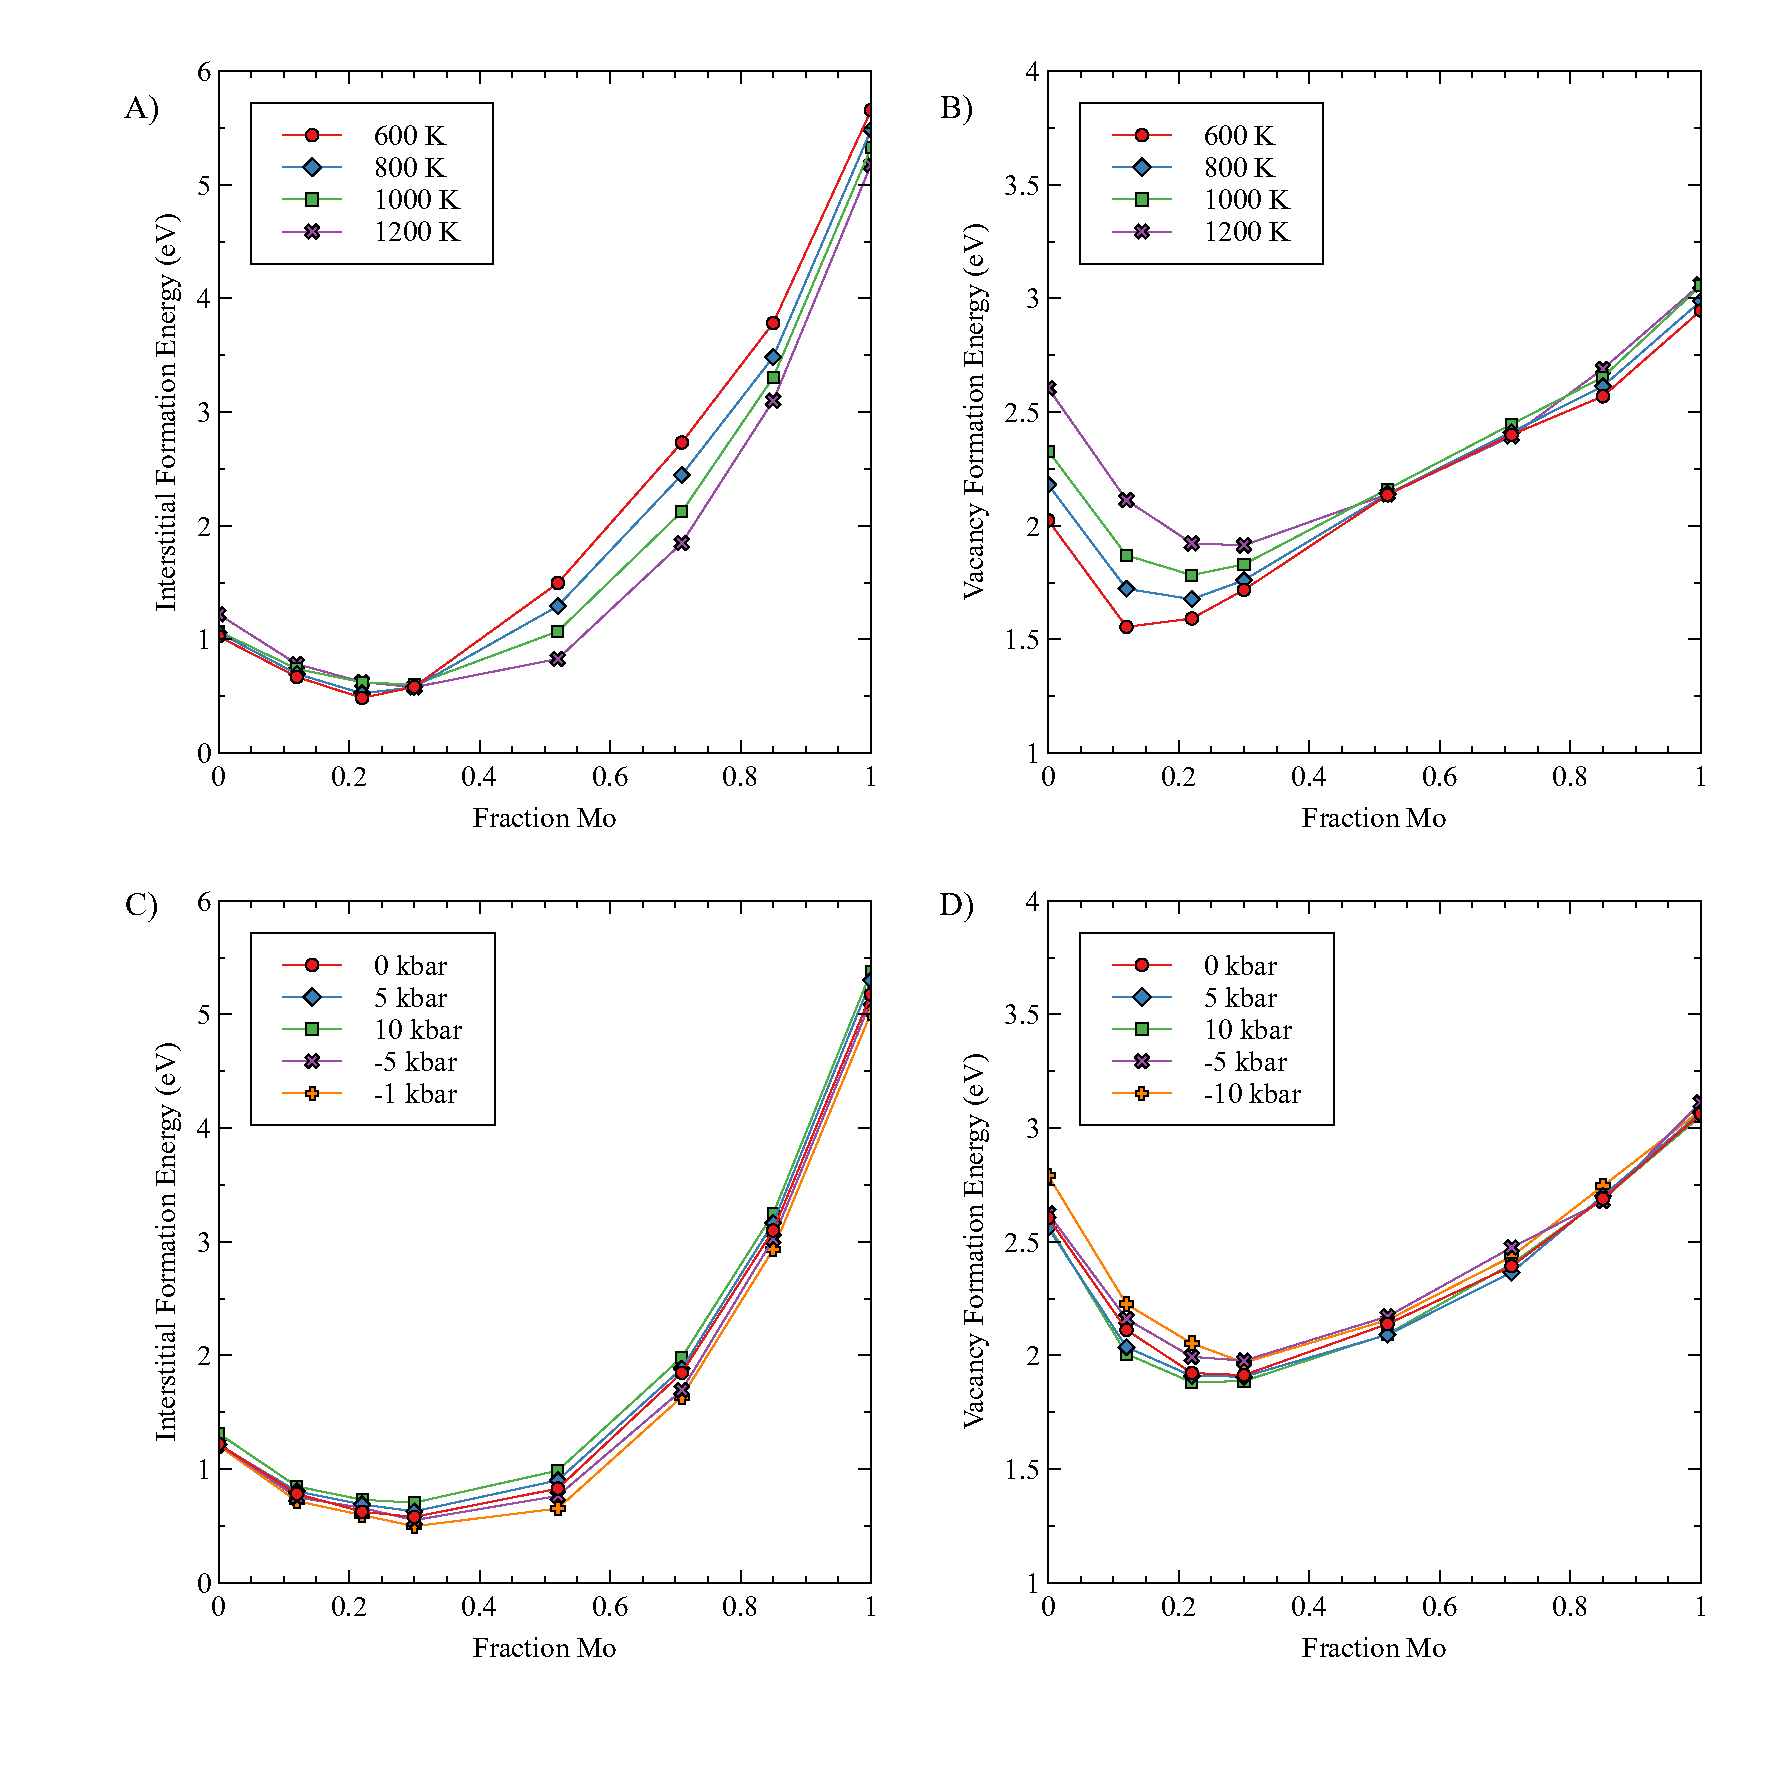
\includegraphics[width=0.9\textwidth]{figA.pdf} 
\caption{The variation of point defect formation energies in U-Mo as a function of composition, temperature, and pressure. A) The interstitial formation energy as a function of composition at four temperatures. B) The vacancy formation energy as a function of composition at four temperatures. C) The interstitial formation energy as a function of composition at five pressures. D) The vacancy formation energy as a function of composition at five pressures. }
\label{fig:A}
\end{center}
\end{figure}

\section{Discussion}\label{sec4}
This work investigated how the hydrostatic tension and compression affect the formation energy of interstitials and vacancies as a function of pressure, temperature and composition in U-Mo. On average, the maximum applied pressure of 10 kbar produces a 6\% increase in the interstitial formation energy and a 3\% decrease in the vacancy formation energy. Under reasonable applied bulk pressures below the yield point ($<$100 MPa), negligible deviations in the defect formations are observed. There are impacts of the applied pressure on defect formation and clear trends can be observed, but these effects are sufficiently small, even at large pressures, that they likely can be neglected for practical purposes. However, in circumstances where the pressures may be quite large, e.g., in the area surrounding a highly pressurized nanometer-sized bubble, statistically significant changes in the local defect formation energy could be observed, potentially altering fission gas bubble evolution and creep behaviors. This work provides the basis for expansion to investigate the effects of applied pressure on defect diffusion, the behavior of defects under a stress gradient, and the generation of point defects due to applied pressure. 

\section{Acknowledgements}\label{sec5}
This work was supported by the U.S. Department of Energy, Office of Material Management and Minimization, National Nuclear Security Administration, under DOE-NE Idaho Operations Office Contract DE-AC07-05ID14517. This manuscript has been authored by Battelle Energy Alliance, LLC with the U.S. Department of Energy. The publisher, by accepting the article for publication, acknowledges that the U.S. Government retains a nonexclusive, paid-up, irrevocable, worldwide license to publish or reproduce the published form of this manuscript, or allow others to do so, for U.S. Government purposes. This research made use of the resources of the High Performance Computing Center at Idaho National Laboratory, which is supported by the Office of Nuclear Energy of the U.S. Department of Energy and the Nuclear Science User Facilities.

\section{Conflict of Interest}\label{sec6}
The authors declare no competing financial interest.

\section{Data Availability}\label{sec7}
Data will be made available upon request to the corresponding author. 

\bibliographystyle{abbrv}
\bibliography{beelerbib}

\end{document}
